\documentclass[a4paper, 12pt]{book}
\usepackage[margin=0.8cm, includefoot, includehead]{geometry}

\usepackage{url}
\usepackage{epsfig}
\usepackage{graphics}

\usepackage{fancyhdr}
\fancyhf{} % clear all header and footers
\renewcommand{\headrulewidth}{0pt} % remove the header rule
\fancyhead[R]
{
	\ifodd\value{page}
		\thepage
	\else
		\hfill
	\fi
}
\fancyfoot[R]
{
	\ifodd\value{page}
		\hfill
	\else
		\thepage
	\fi
}

\pagestyle{fancy}
\fancypagestyle{plain}{%
	\fancyhf{}%
	\renewcommand{\headrulewidth}{0pt}%
	\fancyhead[R]
	{
		\ifodd\value{page}
			\thepage
		\else
			\hfill
		\fi
	}
	\fancyfoot[R]
	{
		\ifodd\value{page}
			\hfill
		\else
			\thepage
		\fi
	}
}

\usepackage{graphicx}
\usepackage{parskip}
\usepackage[utf8]{inputenc}
\usepackage{float}
\usepackage{subcaption}
\usepackage[numbers]{natbib}
\usepackage{algorithm}
\usepackage[noend]{algpseudocode}
\usepackage{amsmath}
\usepackage[numbib,nottoc]{tocbibind}
\usepackage[table,xcdraw]{xcolor}
\usepackage{multirow}
\usepackage[brazil]{babel}
\usepackage[pages=some]{background}
\usepackage{afterpage}
\usepackage{color}
\usepackage{kantlipsum}
\usepackage[sfdefault,light]{roboto}  %% Option 'sfdefault' only if the base font of the document is to be sans serif
\usepackage[T1]{fontenc}
\usepackage{multicol}

\usepackage[toc]{multitoc}
\renewcommand*{\multicolumntoc}{2}
% \setlength{\columnseprule}{0.5pt}

\usepackage{hyperref}
\hypersetup{
    colorlinks,
    citecolor=black,
    filecolor=black,
    linkcolor=black,
    urlcolor=black
}

\usepackage{tikz}
\usetikzlibrary{calc}

\usepackage{tocloft}

\setlength{\cftbeforesecskip}{2pt}

\definecolor{section_color}{RGB}{227, 170, 84}
\definecolor{other_color}{RGB}{125, 87, 68}

\newcommand*{\sectioncolor}{section_color}
\newcommand*{\sectionformat}{\color{\sectioncolor}}

\graphicspath{{pictures/}}

\backgroundsetup
{
	scale = 1,
	color = black,
	opacity = 1.0,
	angle = 0,
	contents = 
	{
  		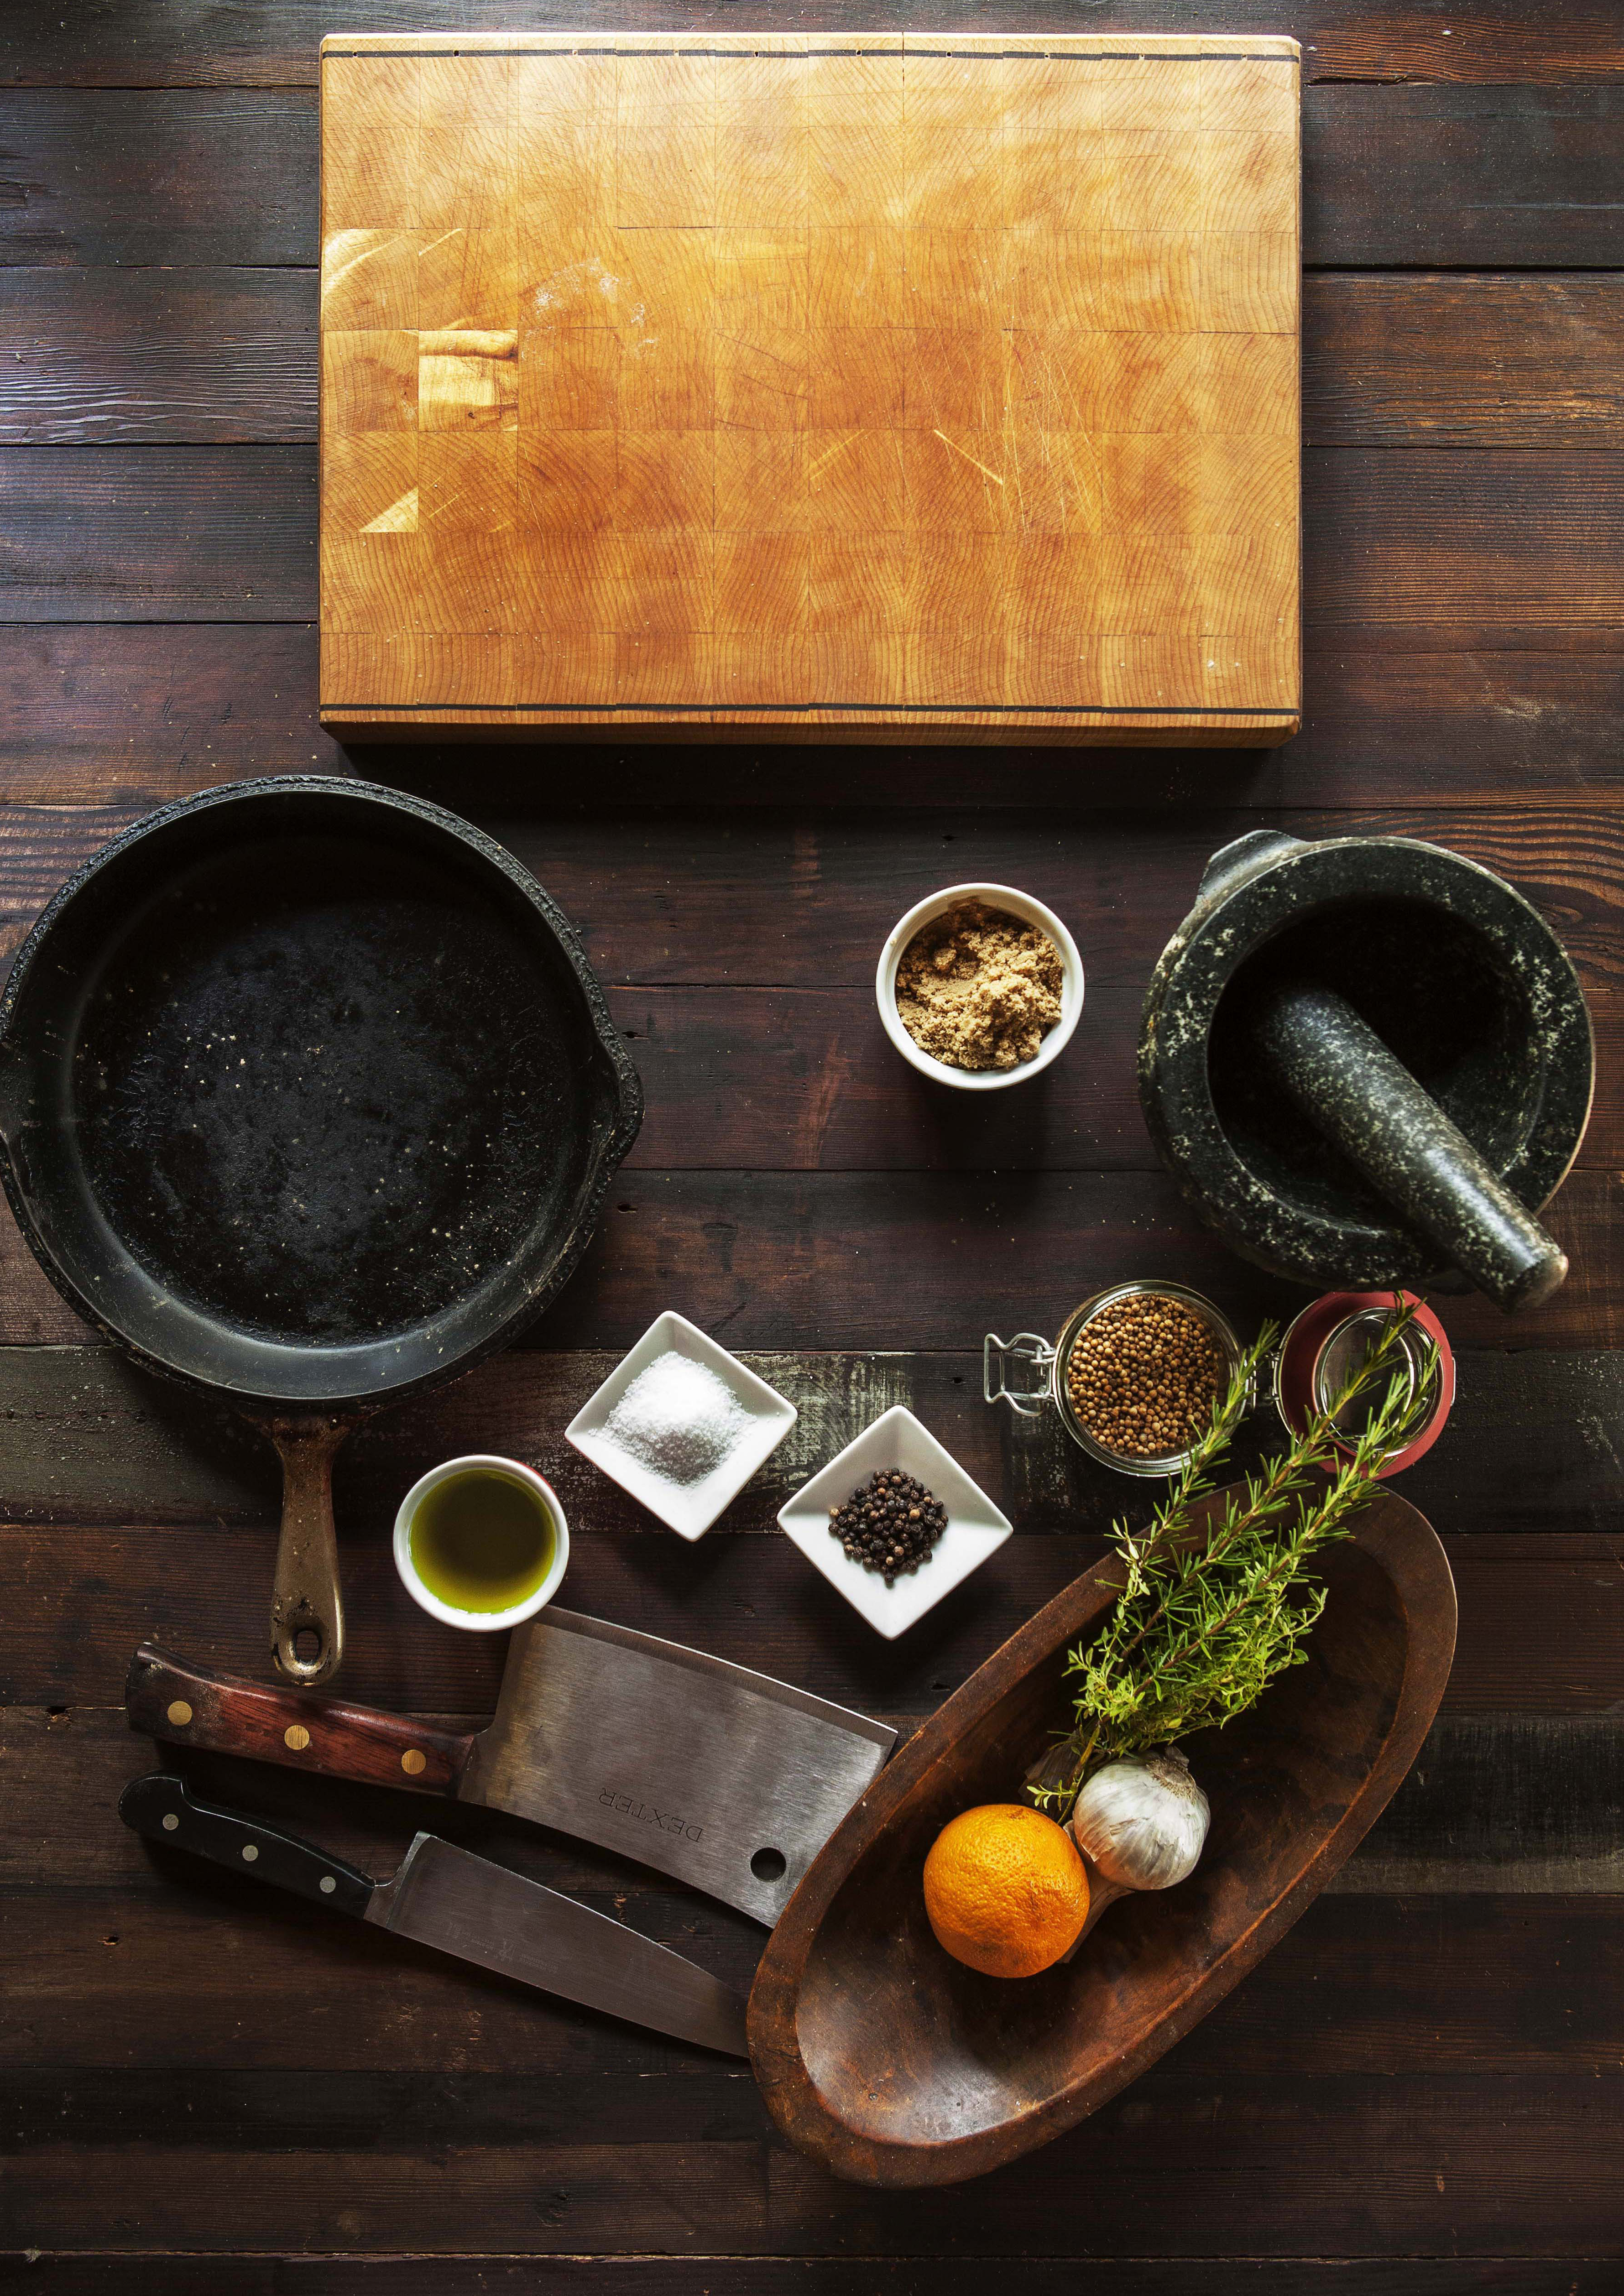
\includegraphics[width=\paperwidth,height=\paperheight]{cover.jpg}
  	}
}

\title
{
	\vspace*{-12.8cm}
	\scalebox{1.0}
	{
		\textbf{E aí, como estamos de macarrão?}
	}
	\scalebox{0.7}
	{
		Um guia de receitas que deram certo
	}
}
\author{
	\\[2.4cm]
	\centering
	\scalebox{1.0}
	{
	    \begin{tabular}{cc}
			\multicolumn{2}{c}{
				Cobaias
			}
			\\[0.15cm]
			\multicolumn{2}{c}{
				Leila Barreto \& Thiago Lobo
			}
		\end{tabular}
	}
}
\date{}

% \pagestyle{fancy}
% % \setlength{\headheight}{10pt}
% \fancyhead{}
% \fancyfoot{}
% % \lhead{Plano de Negócios - Organização das Indústrias}
% % \rhead{Grupo Fly}
% % \cfoot{\thepage}

\begin{document}
	\BgThispage
	\maketitle
		
	\newpage
	\vspace*{-3cm}
	\tableofcontents
	
	\newpage
\noindent
\begin{minipage}[t][.5\textheight][t]{\textwidth}
	\vspace*{-1cm}
	\section*{\sectionformat Nome da Receita}
	\addcontentsline{toc}{section}{Nome da Receita}
	\vspace*{-0.8cm}
	\begin{multicols}{2}
		\kant[1-3]
	\end{multicols}
\end{minipage}
\begin{tikzpicture}[remember picture, overlay]
\node[anchor = south, inner sep = 0pt, outer sep = 0pt] at (current page.south) 
{
	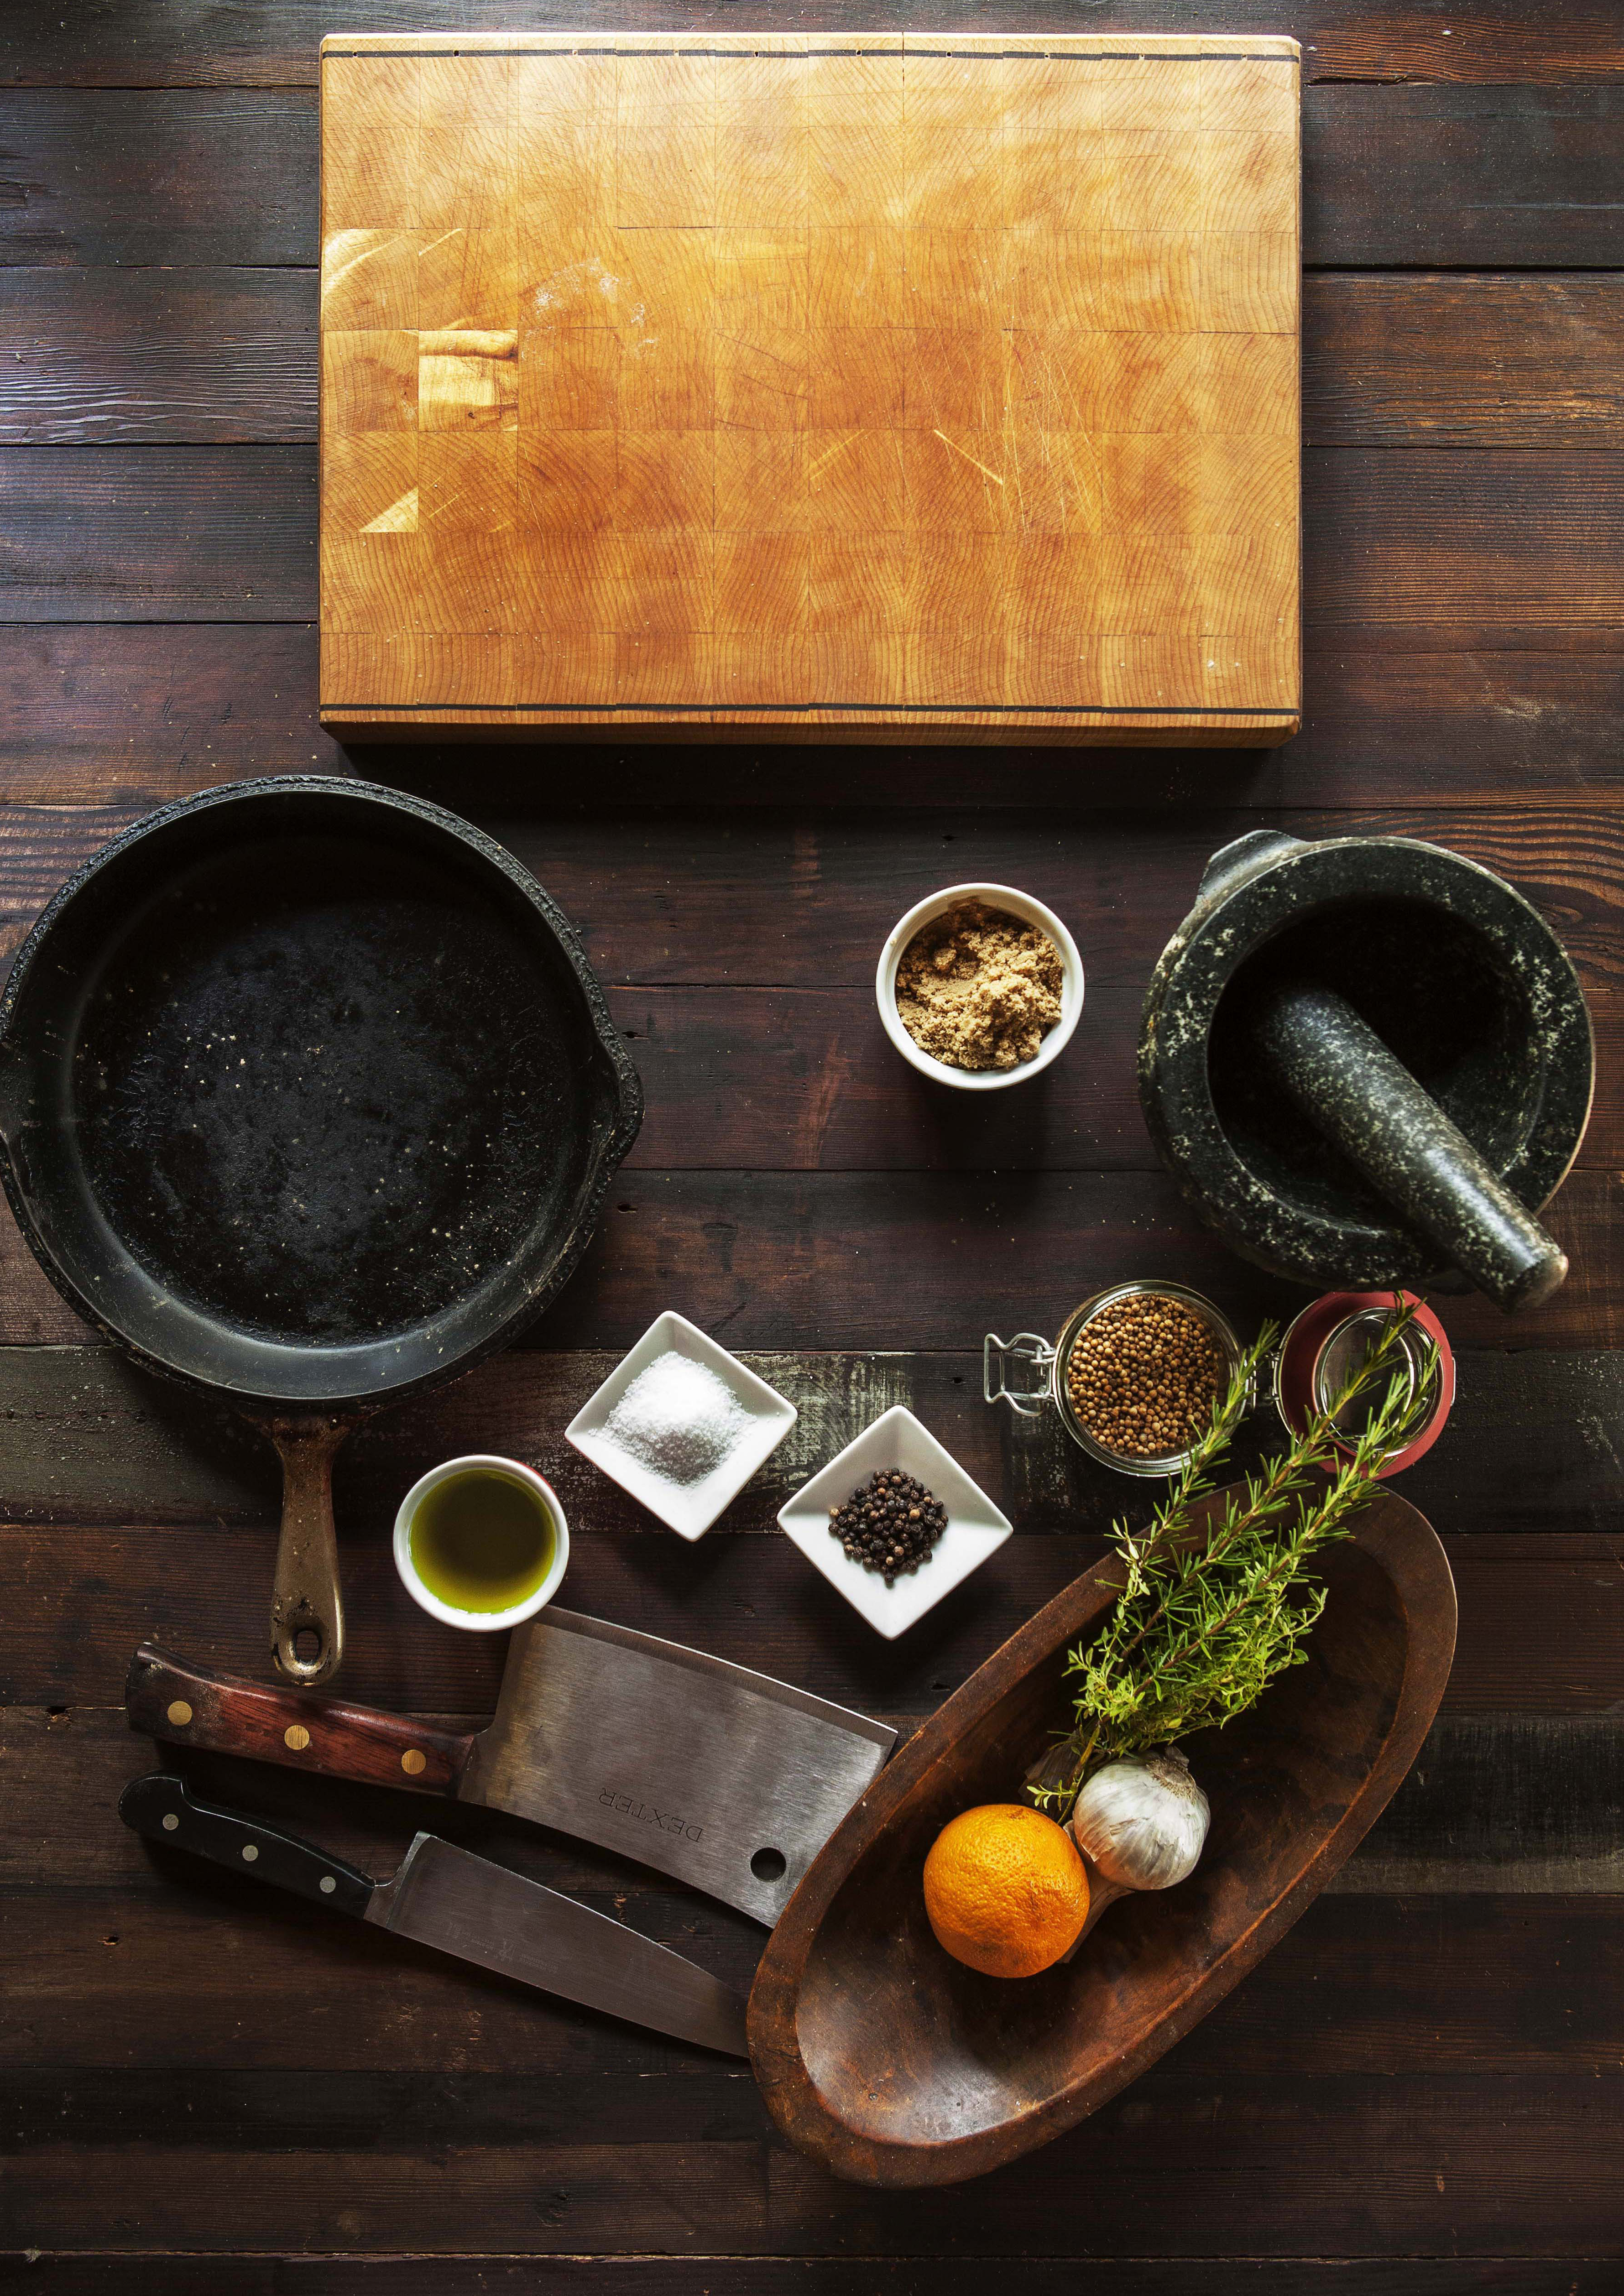
\includegraphics[width=\paperwidth, height=0.45\paperheight]{cover.jpg}
};
\end{tikzpicture}
	% \newpage
\noindent
\begin{minipage}[t]{.5\linewidth}
\section*{Sumário Executivo}
\addcontentsline{toc}{section}{Sumário Executivo}
\kant[1]
\rule{\textwidth}{0.4pt}
\kant[2]

\end{minipage}
\begin{tikzpicture}[remember picture, overlay]
\node[anchor = north east, inner sep = 0pt, outer sep = 0pt] at (current page.north east) 
{
	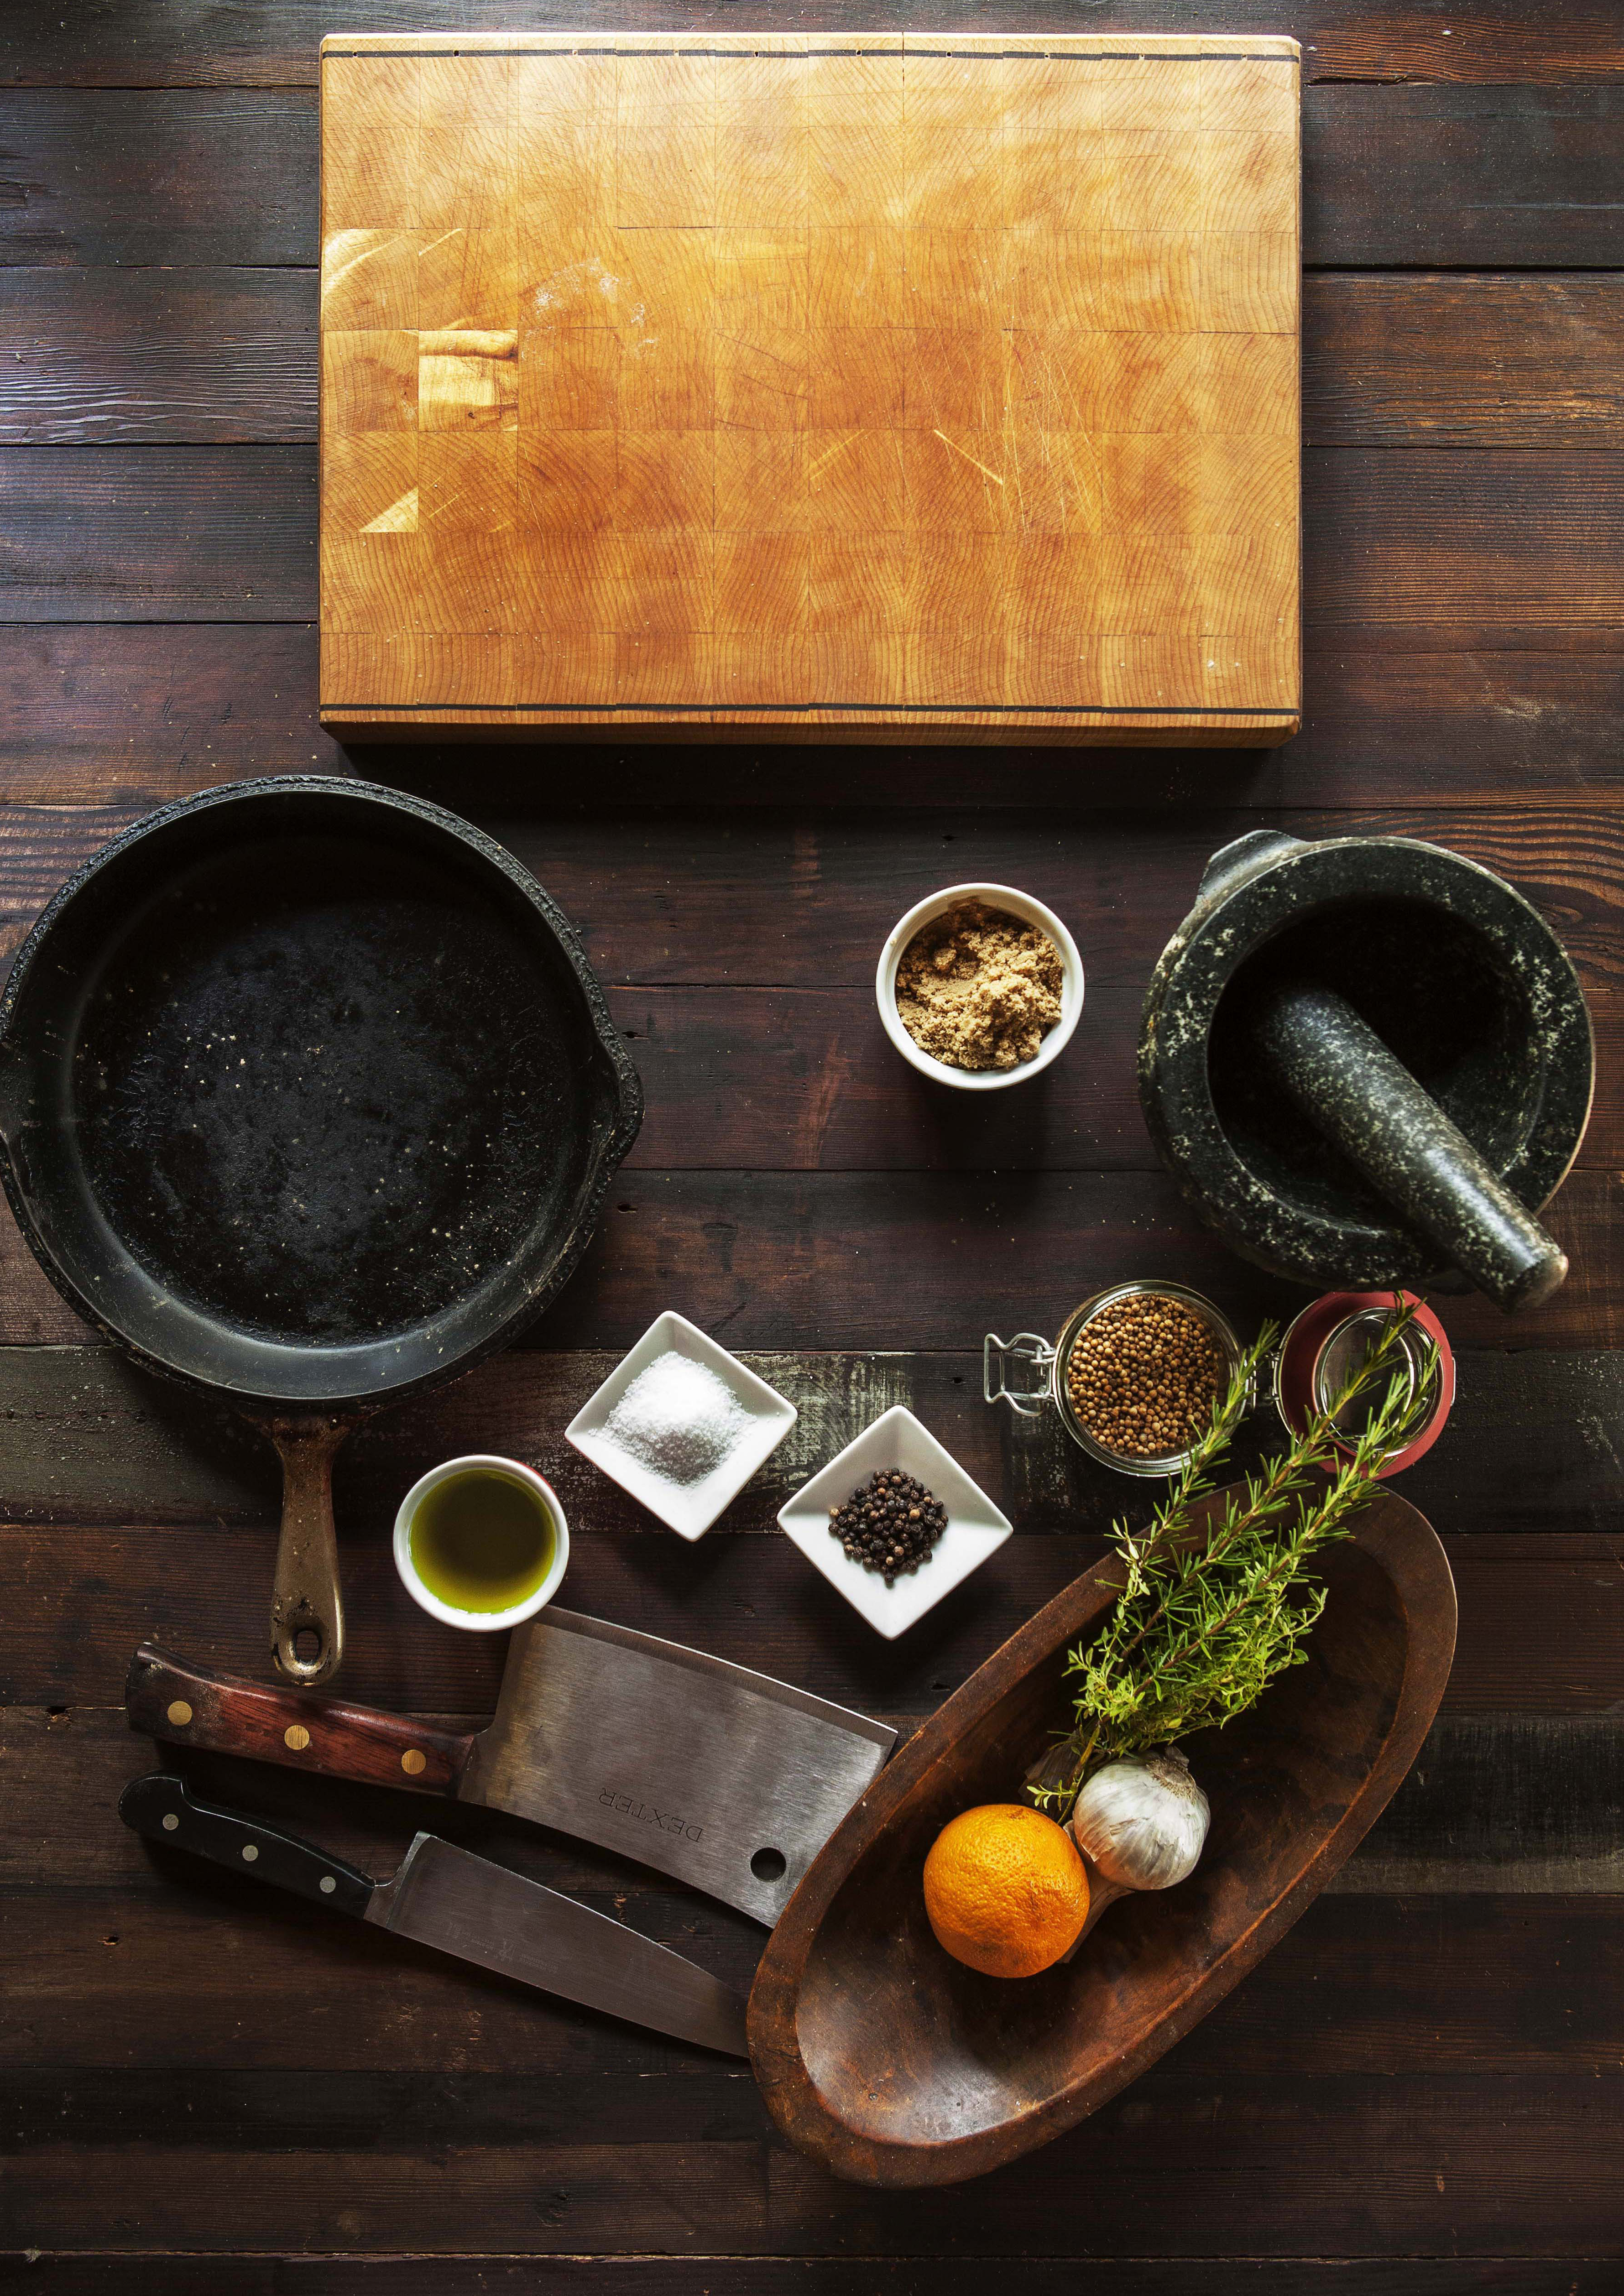
\includegraphics[width=0.45\paperwidth,height=\paperheight]{cover.jpg}
};
\end{tikzpicture}
	\newpage
\noindent
\begin{tikzpicture}[remember picture, overlay]
\node[anchor = north, inner sep = 0pt, outer sep = 0pt] at (current page.north) 
{
	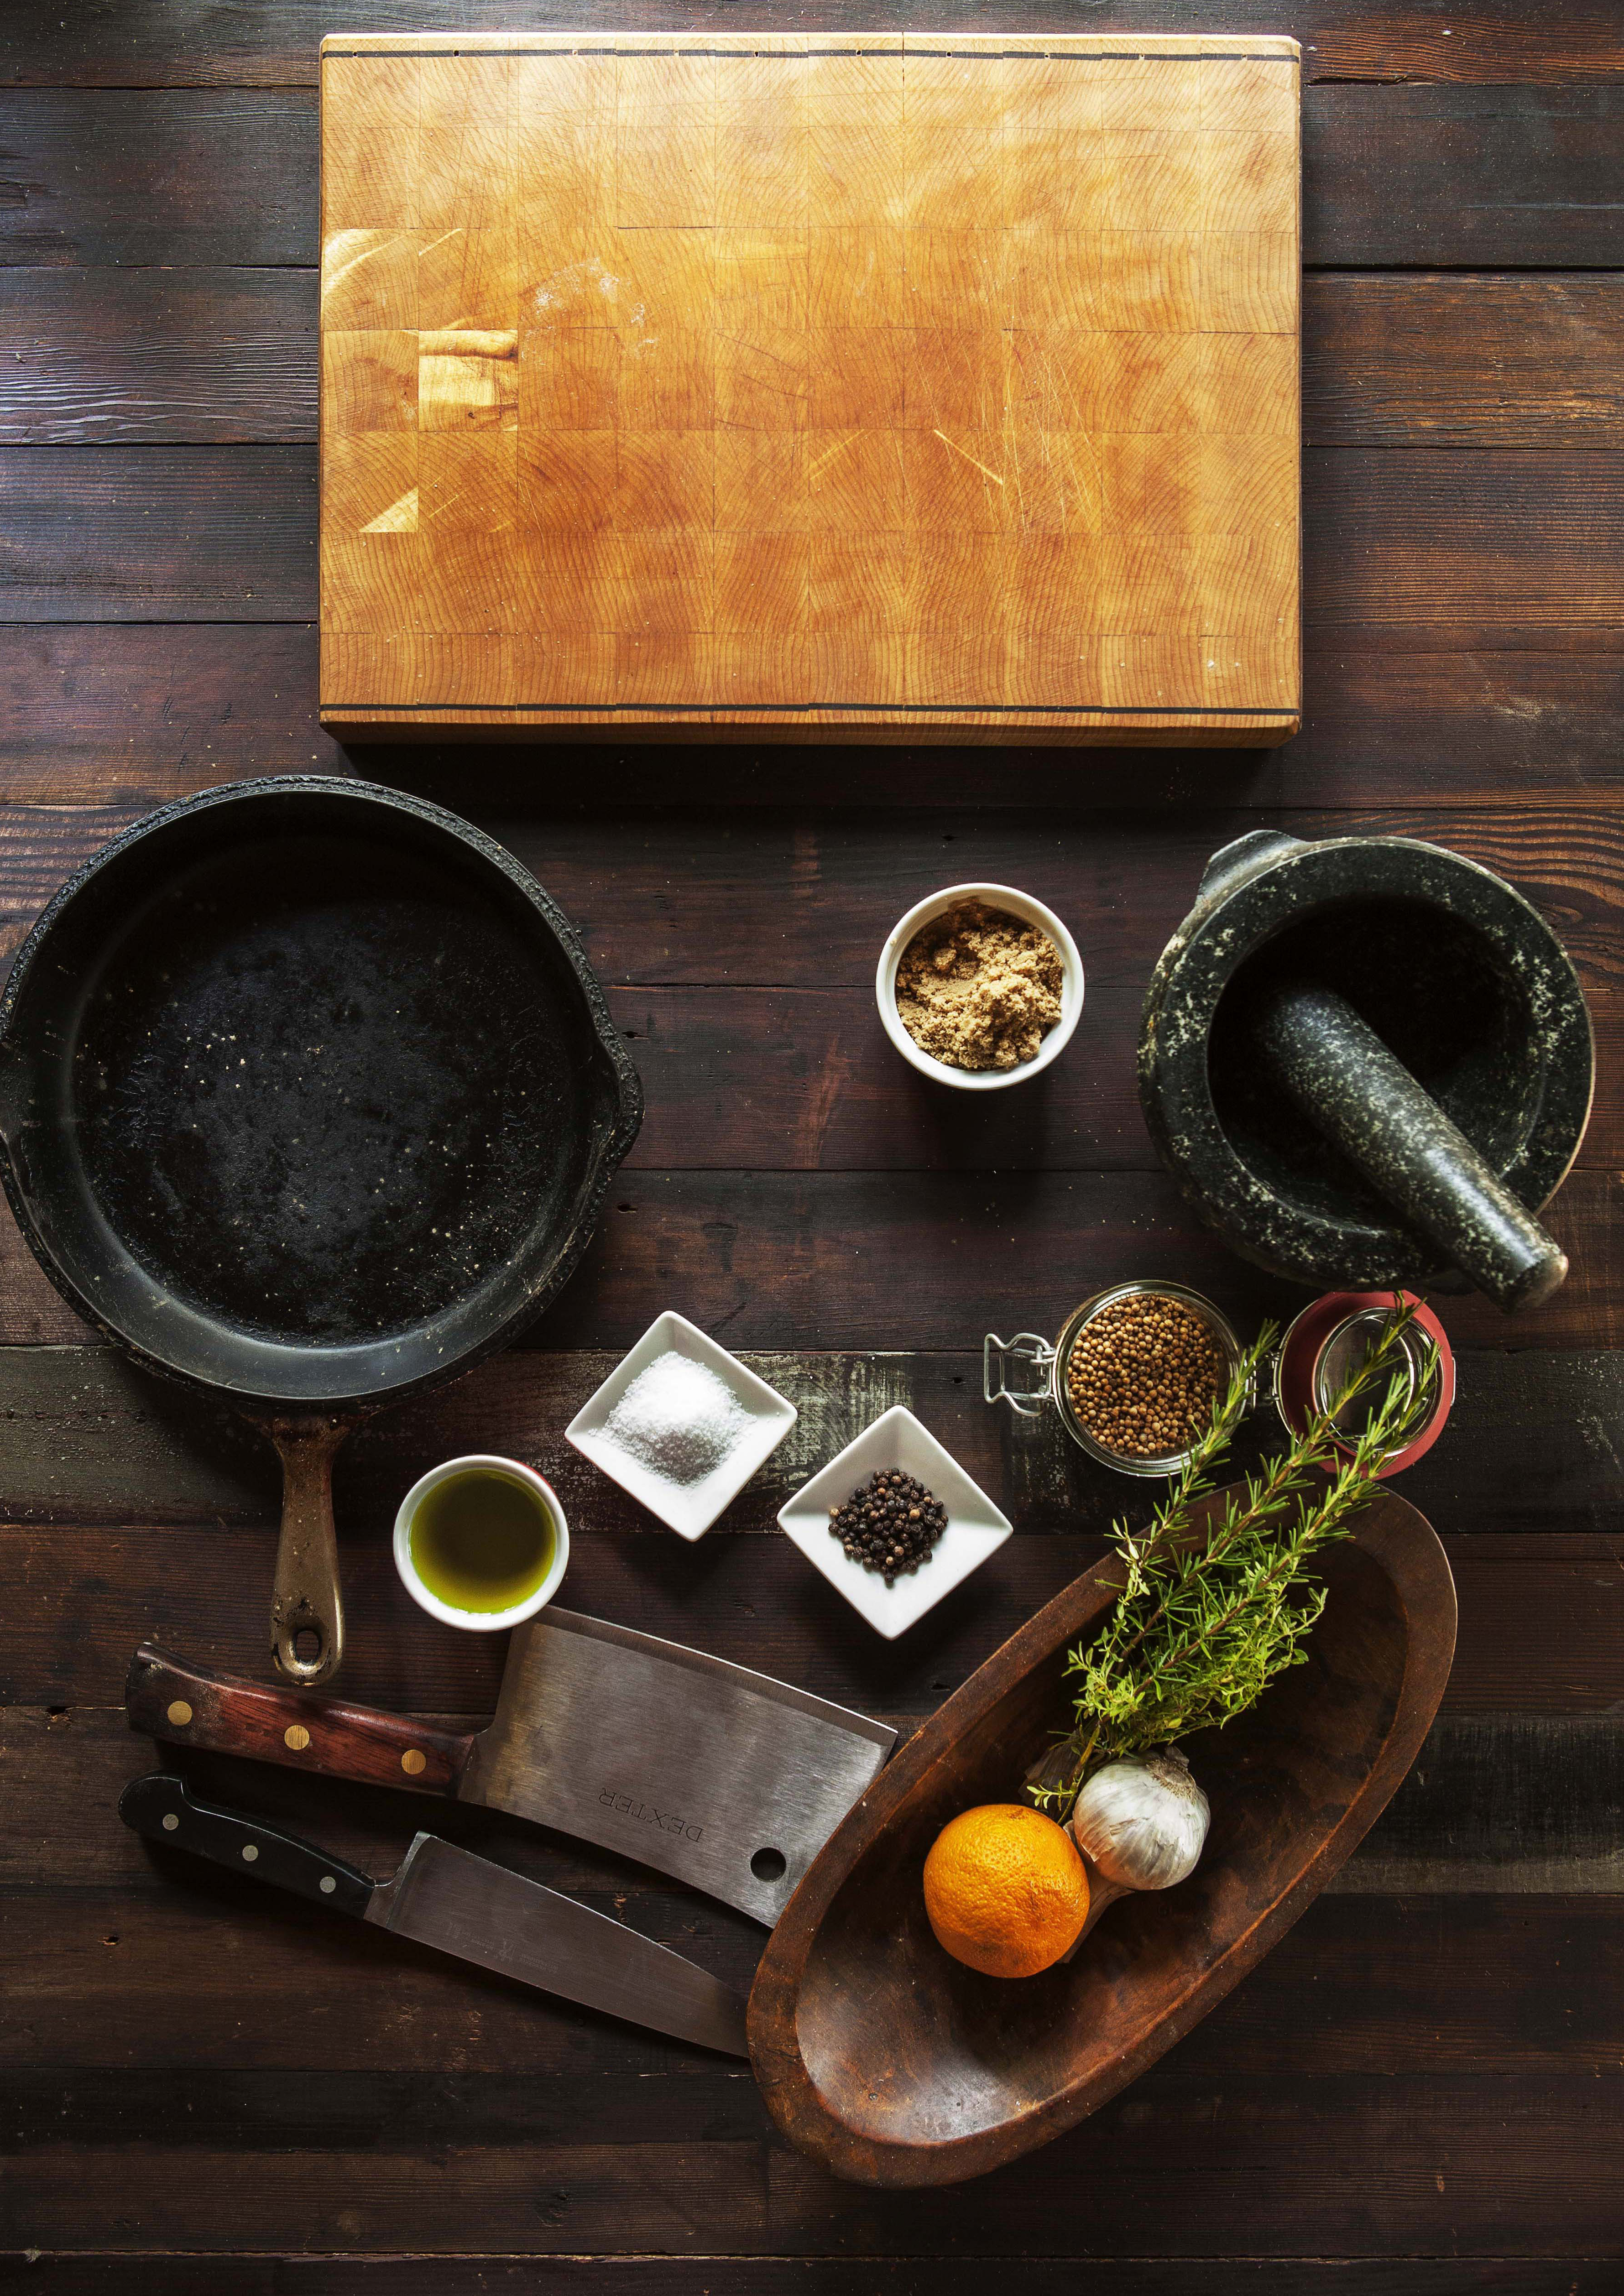
\includegraphics[width=\paperwidth, height=0.45\paperheight]{cover.jpg}
};
\end{tikzpicture}
\begin{minipage}[t][0.5\textheight][t]{\textwidth}
	\vspace*{0.4\paperheight}
	\section*{\sectionformat Nome da Receita}
	\addcontentsline{toc}{section}{Nome da Receita}
	\begin{multicols*}{2}
		\hspace*{-0.28cm}
		\begin{tabu} to 1.04\linewidth {X[l]X[r]}
		   \textit{Serve $3$ pessoas} & \textit{$430$ kcal}
		\end{tabu}\\
		\rule[0.5ex]{\linewidth}{1pt}
		\subsection*{\subsectionformat Teste}
		% \vspace*{-0.8cm}
		\kant[1]
	\end{multicols*}
\end{minipage}

	\newpage
\noindent
\begin{minipage}[t][.5\textheight][t]{\textwidth}
	\vspace*{-1cm}
	\section*{\sectionformat Nome da Receita}
	\addcontentsline{toc}{section}{Nome da Receita}
	\vspace*{-0.8cm}
	\begin{multicols}{2}
		\kant[1-3]
	\end{multicols}
\end{minipage}
\begin{tikzpicture}[remember picture, overlay]
\node[anchor = south, inner sep = 0pt, outer sep = 0pt] at (current page.south) 
{
	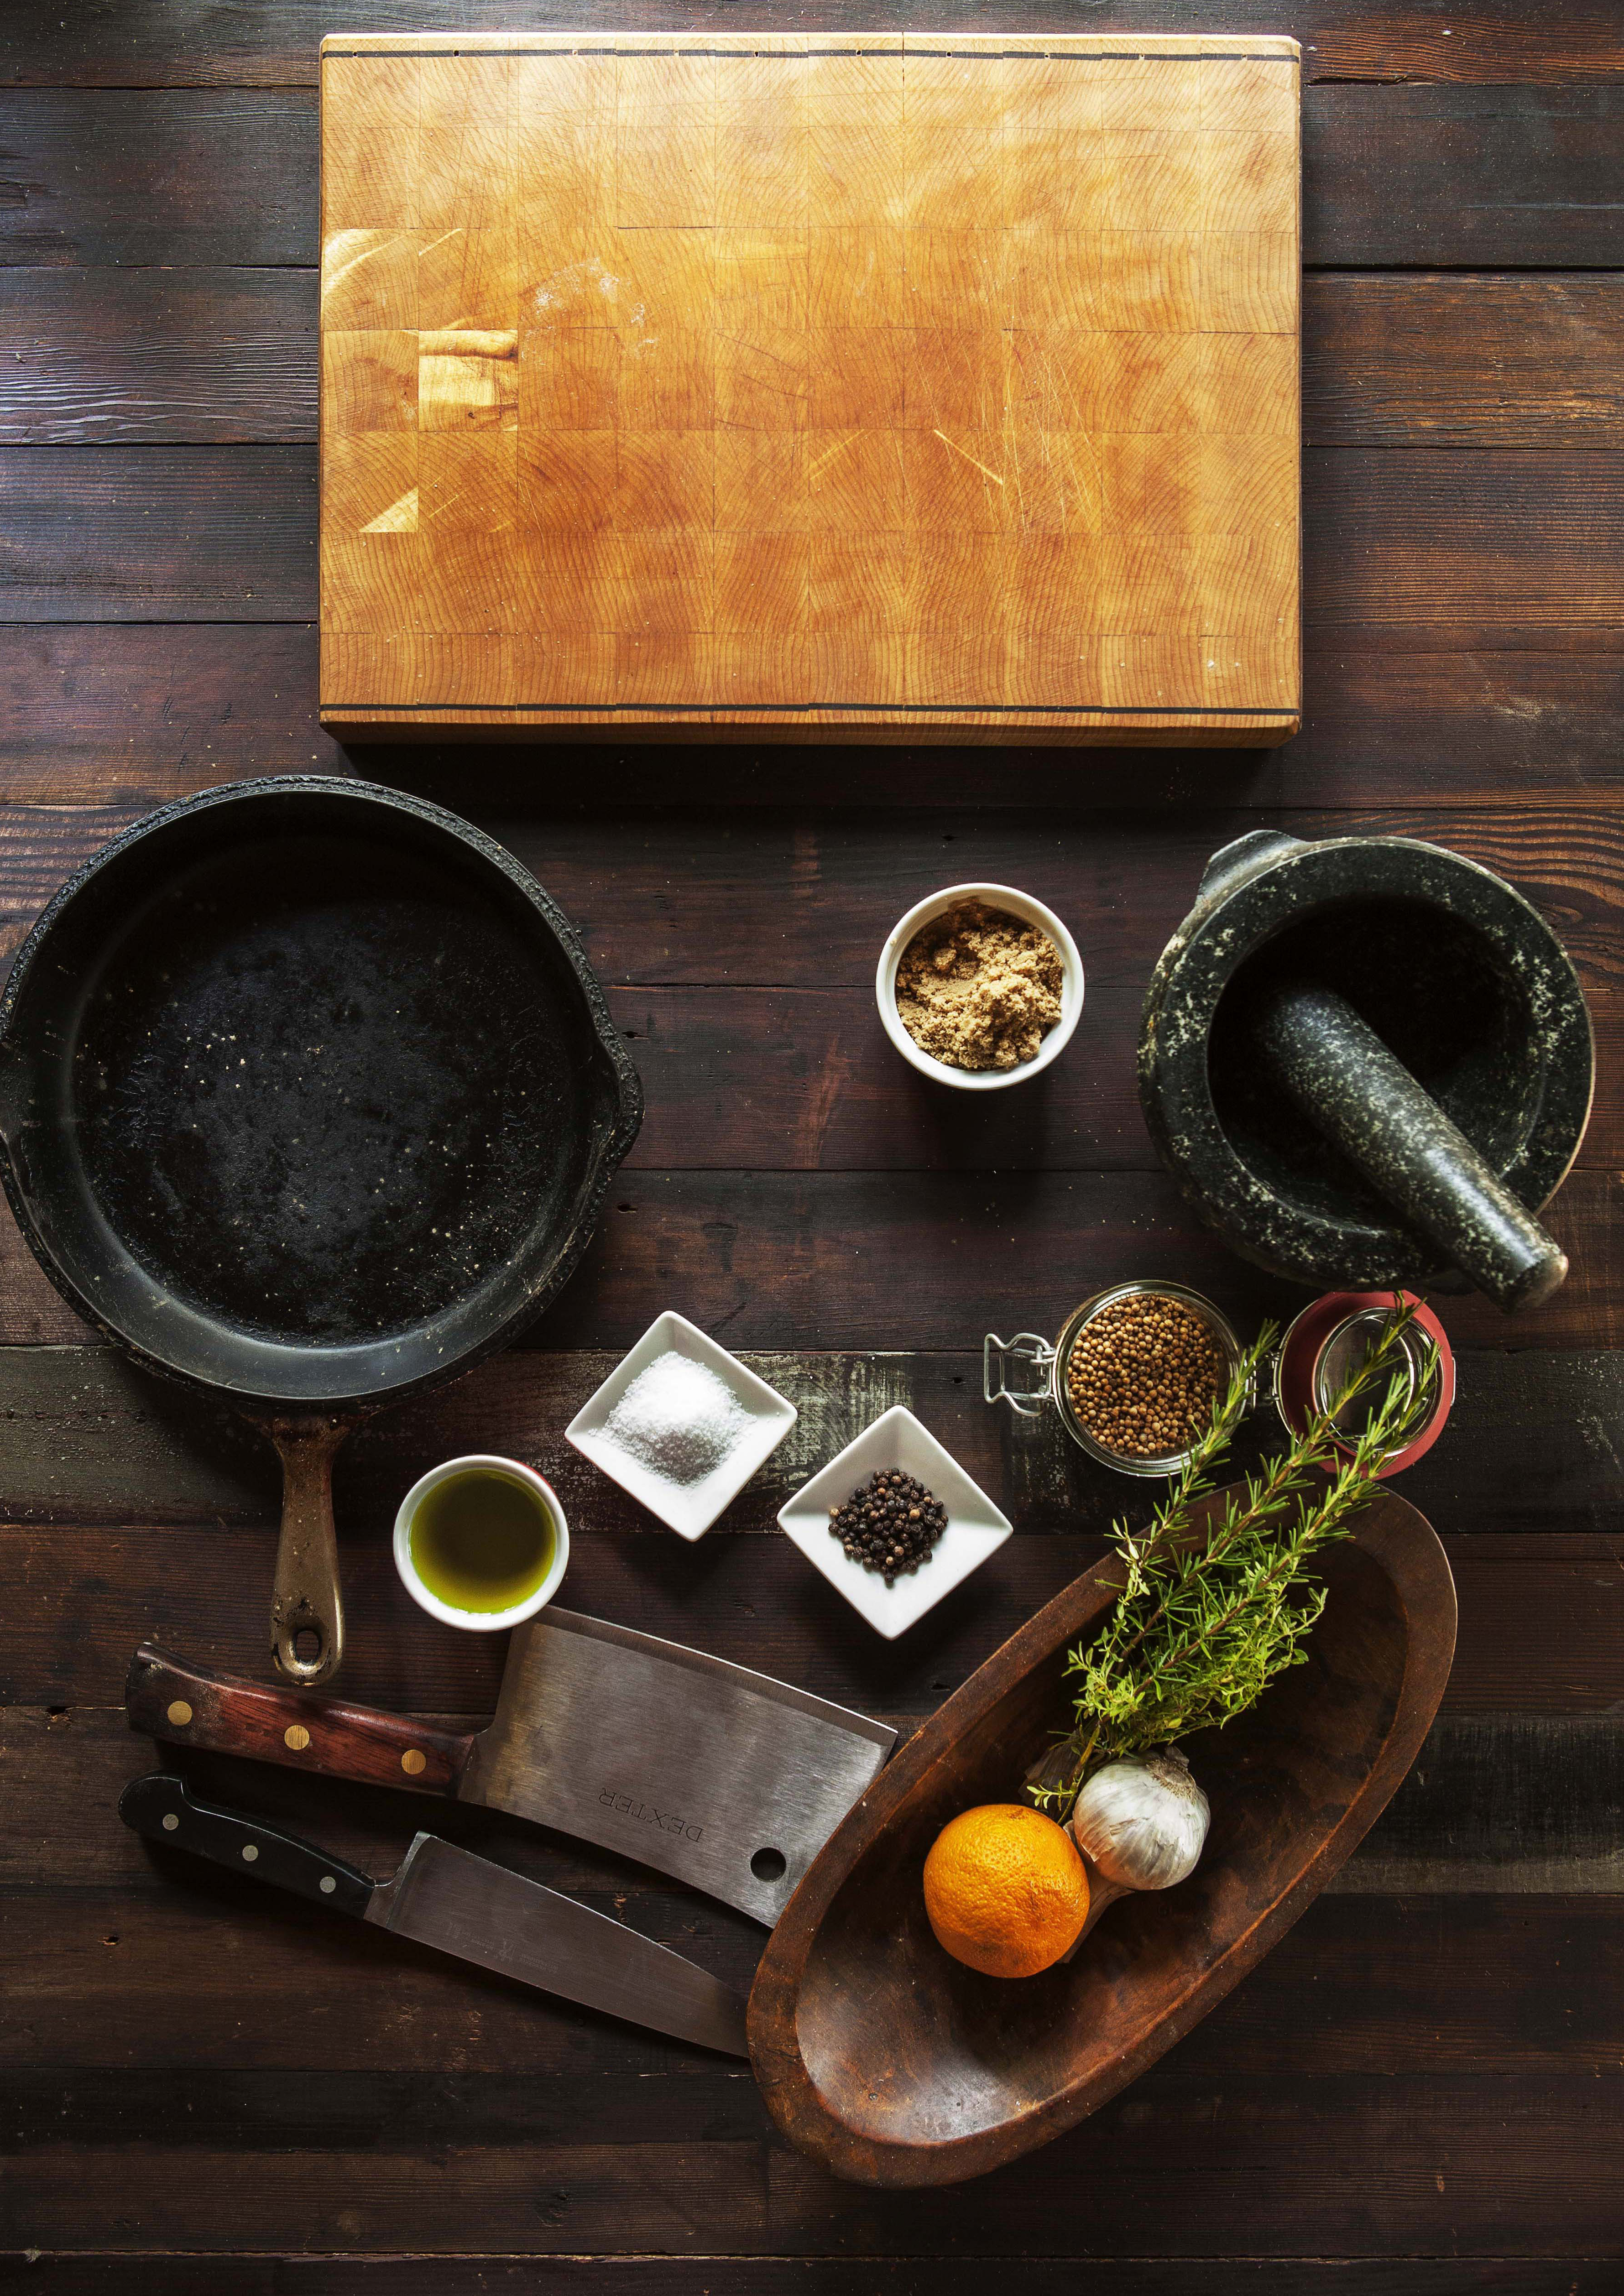
\includegraphics[width=\paperwidth, height=0.45\paperheight]{cover.jpg}
};
\end{tikzpicture}
	\newpage
\noindent
\begin{tikzpicture}[remember picture, overlay]
\node[anchor = north, inner sep = 0pt, outer sep = 0pt] at (current page.north) 
{
	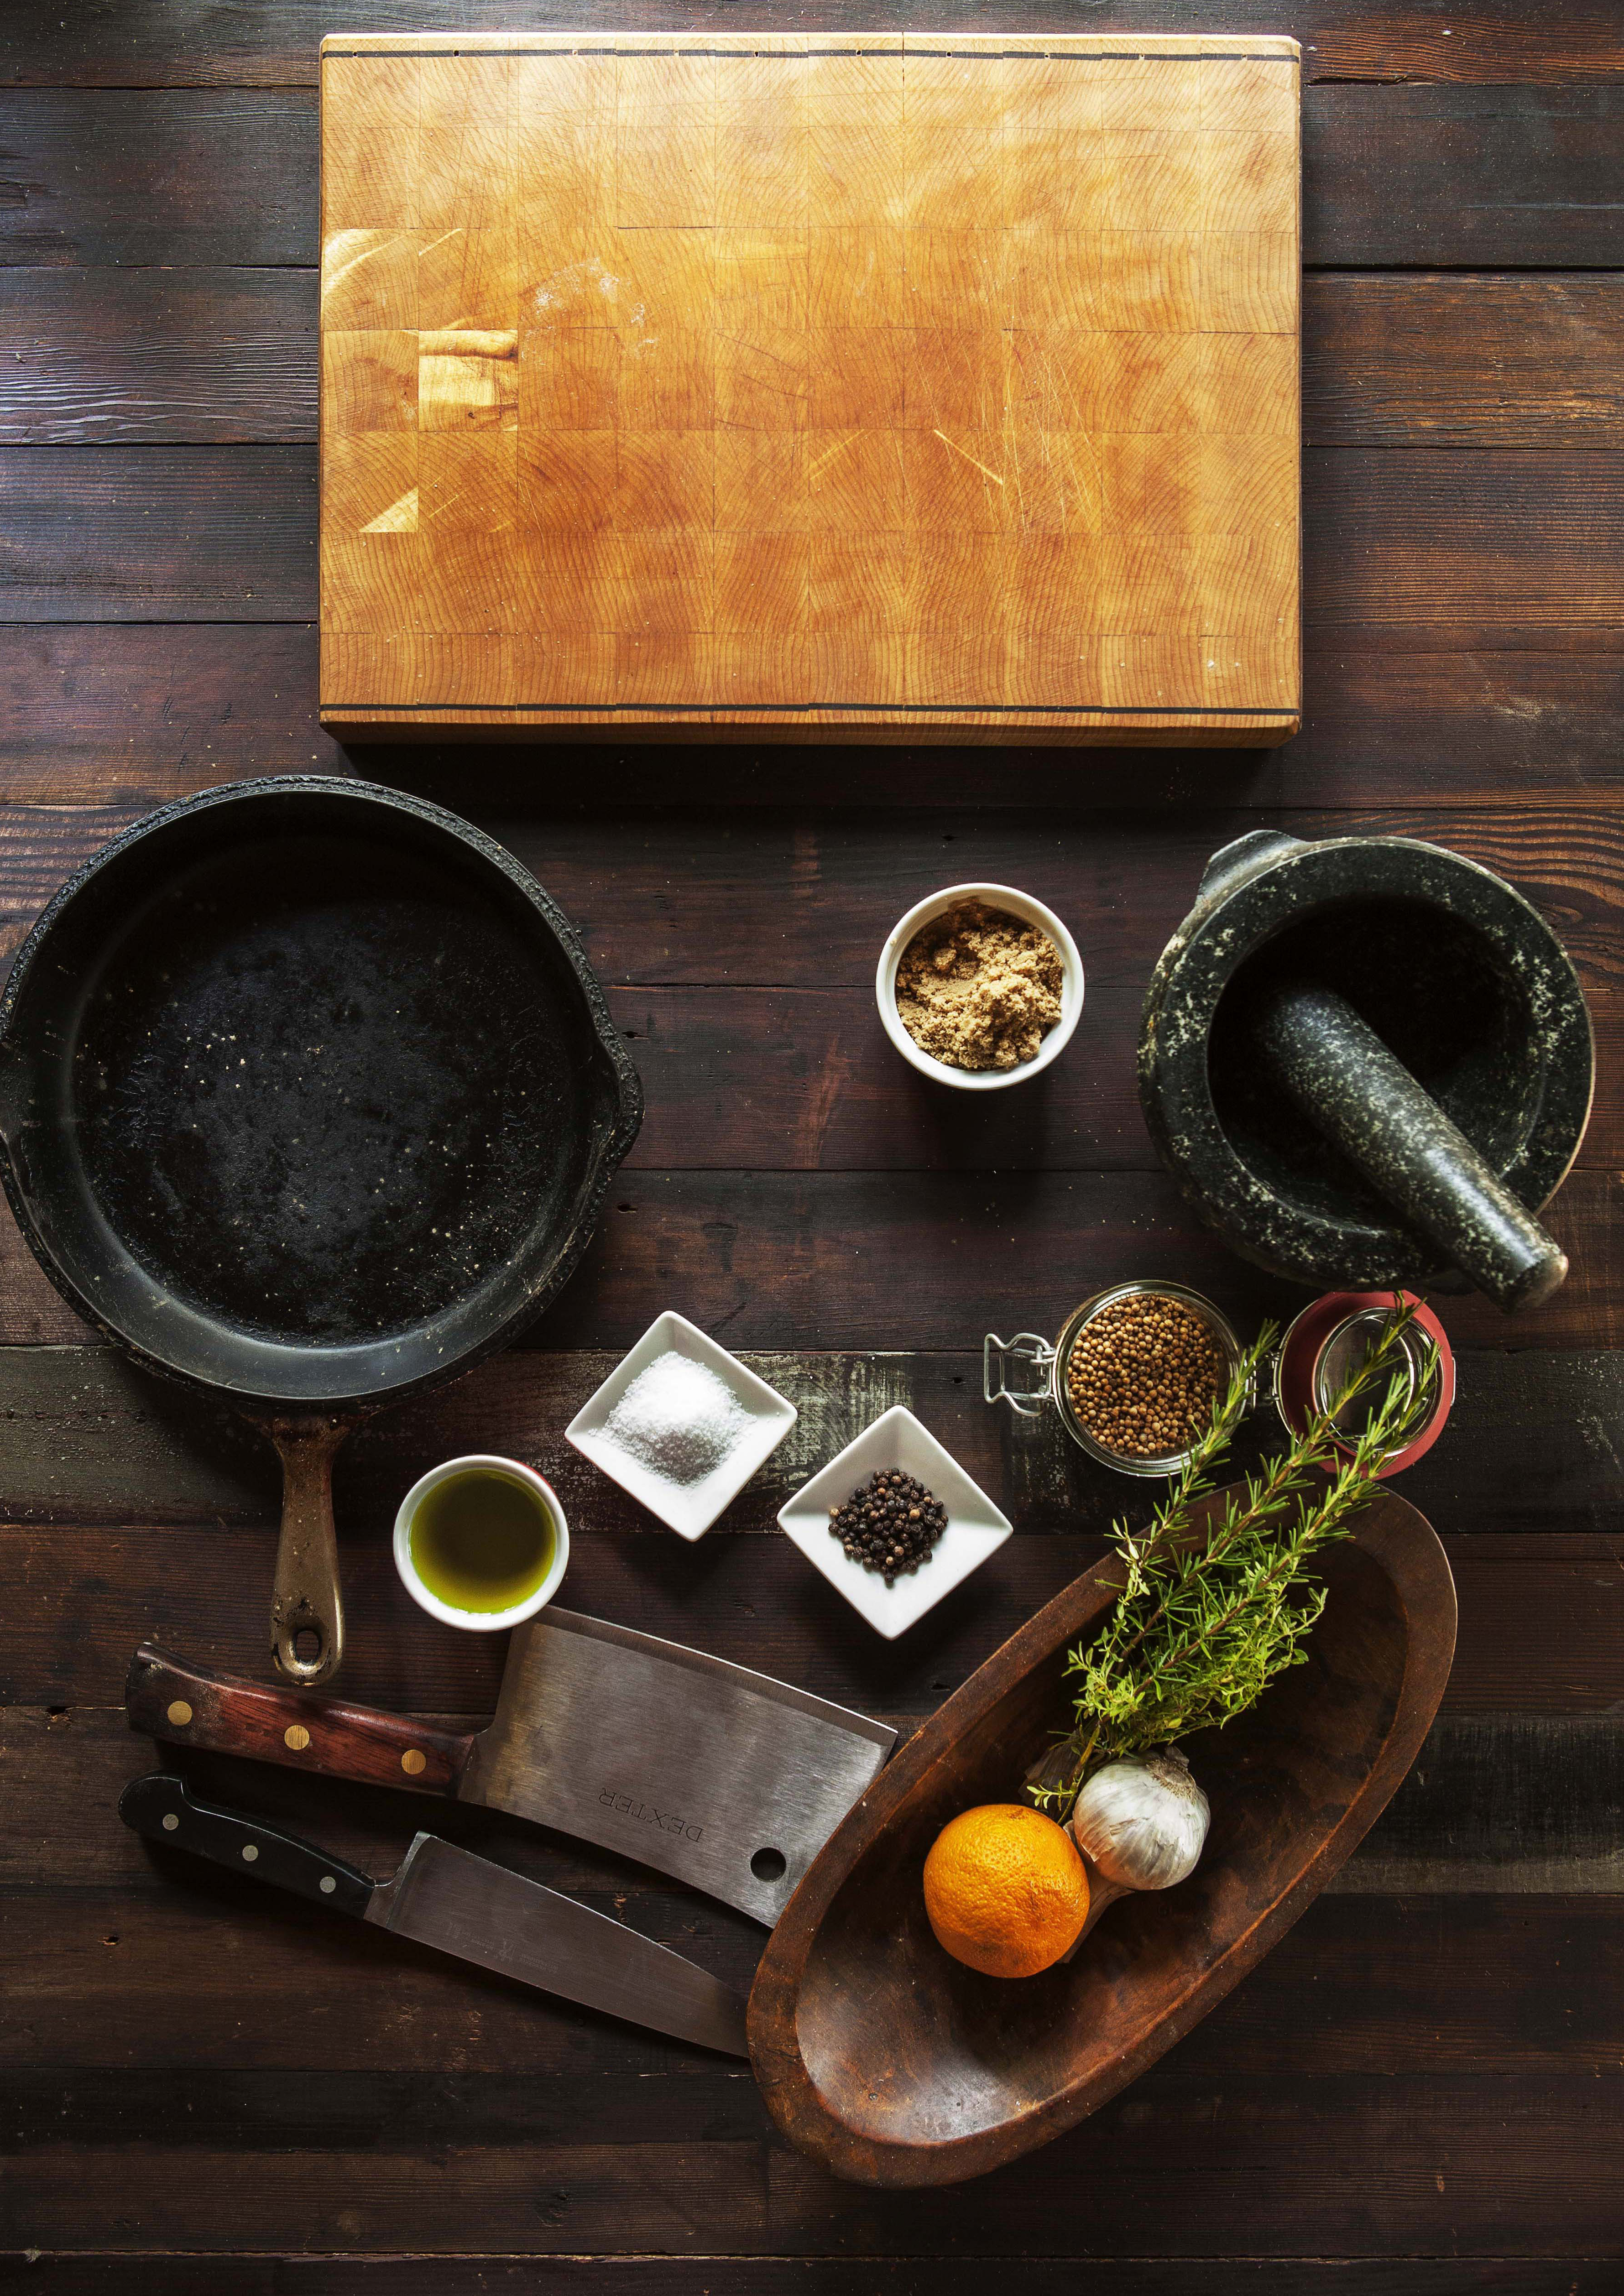
\includegraphics[width=\paperwidth, height=0.45\paperheight]{cover.jpg}
};
\end{tikzpicture}
\begin{minipage}[t][0.5\textheight][t]{\textwidth}
	\vspace*{0.4\paperheight}
	\section*{\sectionformat Nome da Receita}
	\addcontentsline{toc}{section}{Nome da Receita}
	\begin{multicols*}{2}
		\hspace*{-0.28cm}
		\begin{tabu} to 1.04\linewidth {X[l]X[r]}
		   \textit{Serve $3$ pessoas} & \textit{$430$ kcal}
		\end{tabu}\\
		\rule[0.5ex]{\linewidth}{1pt}
		\subsection*{\subsectionformat Teste}
		% \vspace*{-0.8cm}
		\kant[1]
	\end{multicols*}
\end{minipage}

	% \newpage
\noindent
\hspace*{0.45\paperwidth}
\begin{minipage}[t]{.5\linewidth}
\section*{Sumário Executivo}
\addcontentsline{toc}{section}{Sumário Executivo}
\kant[1-3]
\end{minipage}
\begin{tikzpicture}[remember picture, overlay]
\node[anchor = north west, inner sep = 0pt, outer sep = 0pt] at (current page.north west) 
{
	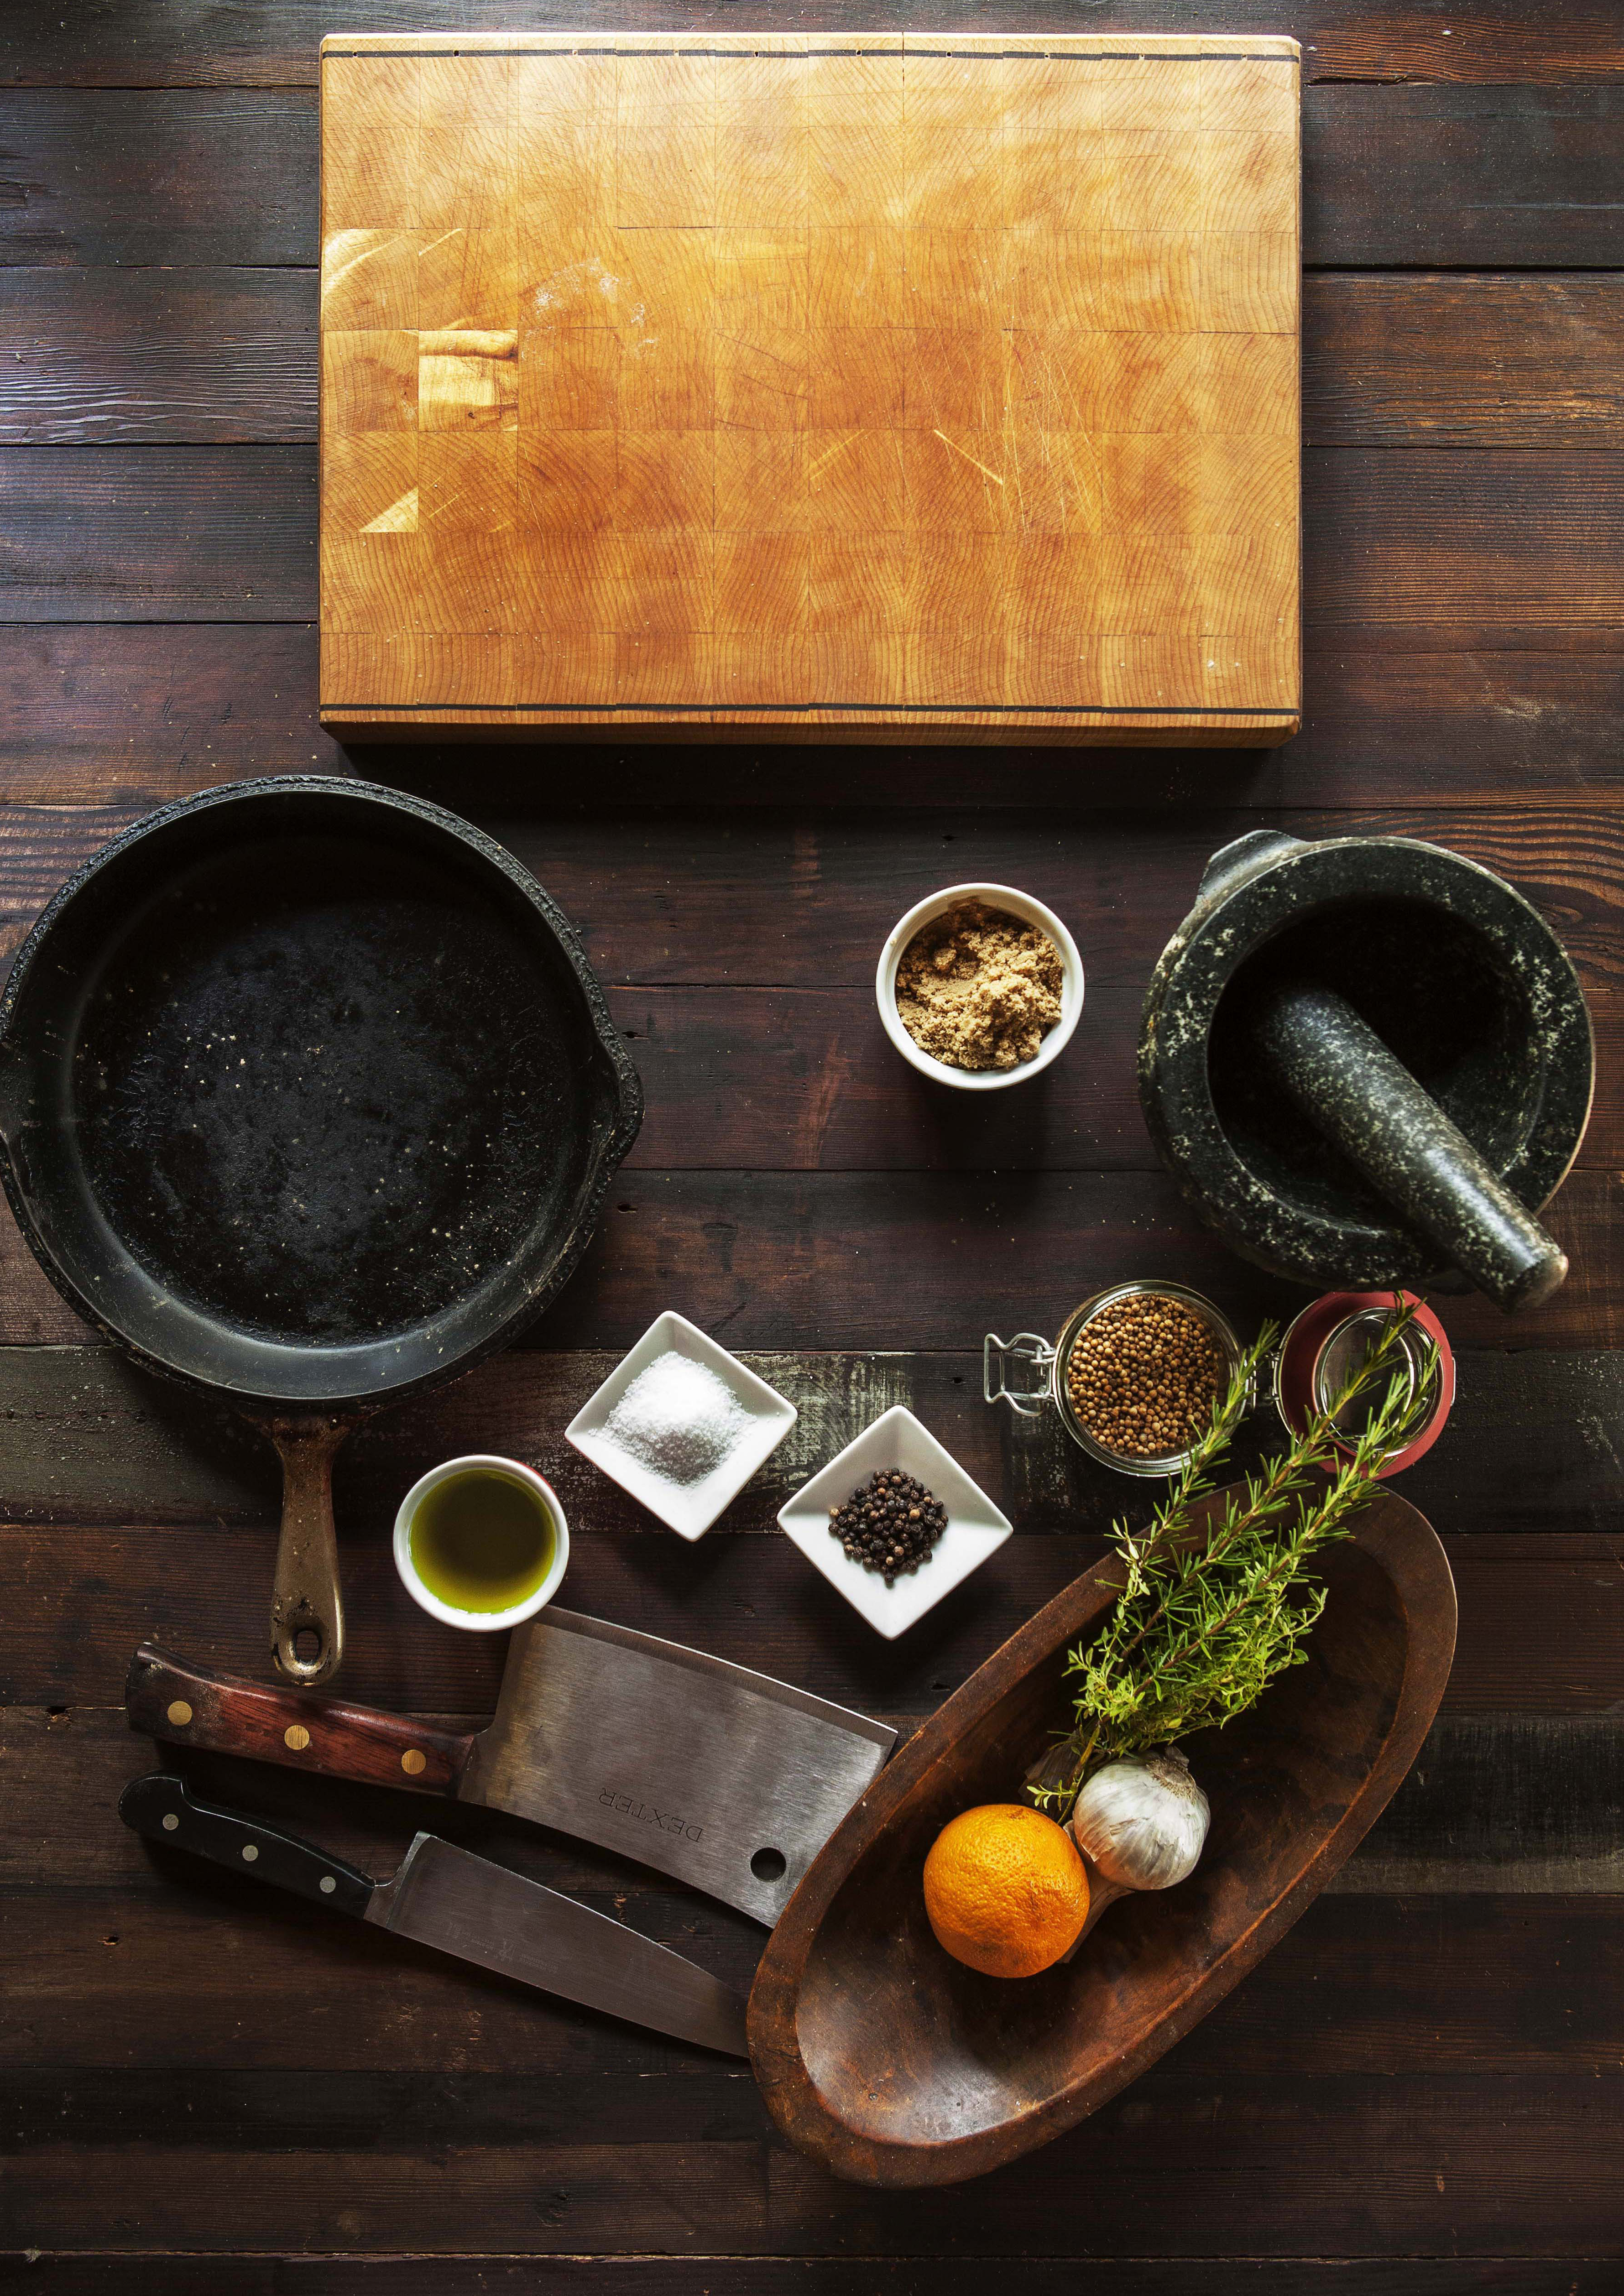
\includegraphics[width=0.45\paperwidth,height=\paperheight]{cover.jpg}
};
\end{tikzpicture}

\end{document}